\documentclass[a4paper,10pt,twocolumn,preprint,3p]{elsarticle}

\usepackage[latin1]{inputenc}
\usepackage{amssymb}
\usepackage{graphicx}
\usepackage{amsmath}
\usepackage{url}
\usepackage{multirow}

\journal{Expert Systems with Applications}

\begin{document}

\begin{frontmatter}

% first the title is needed
\title{Comparing individual representation and evaluation for automatic rule extraction using GP in a BYOD scenario}

\author[ugr]{Paloma De las Cuevas}
\ead{palomacd@ugr.es}
\author[uca]{Pablo Garc\'{\i}a-S\'anchez}
\ead{pablo.garciasanchez@uca.es}
\author[ugr]{J.J. Merelo}
\ead{jmerelo@geneura.ugr.es}
\author[isgt]{Zeineb Chelly}
\ead{zeinebchelly@yahoo.fr}

\address[ugr]{Department of Computer Architecture and Computer Technology, ETSIIT and CITIC \\
University of Granada, Granada, Spain. Tel: +34958241778. Fax: +34958248993}
\address[uca]{Department of Computer Engineering, School of Engineering \\
University of C\'adiz, Spain.}
\address[isgt]{LARODEC, Institut Sup\'erieur de Gestion de Tunis, Tunisia.}


\begin{abstract}
The constant improvement in the computational abilities and features of the personal devices has favoured the application of the concept of ``Bring Your Own Device'' (BYOD) to the corporate world, making the companies to
create policies geared towards enabling these devices as company tools. 
This philosophy allows
employees to bring and use their personal devices at
the company premises, on virtual private networks or otherwise while
on company work. Despite the significant advantages of this policy
such as reducing overheads and increasing work productivity, 
the
access to internal network and the assets it holds by these personal
devices, whose corporate control is forcefully limited, exposes the companies to
security threats such as leak of confidential data and access by
unauthorised users. 
To handle these kinds of threats, we propose a way of detecting and controlling abnormal user
access by establishing a policy based on classification rules. Our
approach for the problem of BYOD security uses Genetic Programming
(GP) via a standard GP framework, since GP is 
capable of discovering of novel and interesting threat classification
rules, with the additional feature of presenting the new rules in an
easily understandable way. % These rules are a re-formulation of the
                           % old rules set by the CSO. They are not totally new - JJ
We obtain good dataset coverage 
after the simulation results over real data, and after testing
different fitness functions and configurations in the way of coding the individuals.
Through these comparisons, we can confirm the 
viability, effectiveness, and applicability of the GP approach, in certain conditions, to the
BYOD security context. 
\end{abstract}


\begin{keyword}
%TODO: Keywords
Bring Your Own Device, Security, Genetic Programming, Rules Extraction. 
\end{keyword}

\end{frontmatter}


\section{Introduction}
\label{sec:intro}

The fast pace of introduction of new technologies has led modern computing to undergo
several outstanding transitions in a short period of time. Modern
computing has moved over time to smaller, more reliable and faster
high-tech devices such as smartphones, laptops and tablets. The use of
these technologies in several forms is progressing, and has led to the
form of use known as the ``Bring Your Own Device'' (BYOD) concept or
philosophy. 
Since its first appearance in research
\cite{ballagas2004byod} as a way to name the interaction between
people's devices and a public display, such as art or advertising, it
has become a very popular practise, integrated into companies
\cite{thomson2012byod} and even schools \cite{song2014bring}.  

In the corporate world, the BYOD
practice refers to allowing employees to use their
personal laptops, smartphones, tablets, and other mobile devices in
for work-related tasks, but not necessarily while being in the workplace This has many
advantages \cite{singh2012byod}; among them we mention saving costs --
since the company saves money on high-priced devices that
it would normally be required to purchase for their employees --, and
increasing flexibility and worker productivity as employees will not
be asked to haul around while on the road multiple devices to satisfy both their personal and
work needs, having everything they need in one device anytime and
anywhere. 
Other advantages are tied to the increase of worker satisfaction, attracting the best candidates, and the increase of engagement in the workplace and after hours \cite{singh2012byod}. 

%These advantages have made BYOD policies gain traction in the education
%sector with an increasing number of schools around the world choosing
%to implement their own BYOD policies. % reference!!! - JJ
% Also I don't see the point. Where do you want to bring this argument to? - JJ
% Ok, maybe we talk too much about BYOD at schools when we use company
% BYOD data, but it's true that schools are environments in which
% policies should be enforced too, right? Or can be applied in another
% way... So, what can we do? To create a section at the end called
% "other applications for our framework", for example? Or just mention
% it, reducing what's written now, and that's all?
% I would go for just mentioning it, because issues are much
% different. What company "assets" are we protecting here? - JJ
%In such environment, BYOD (also called Bring Your Own Technology) refers to a technology model that
%allows students to bring their own devices to school for learning in
%the classroom \cite{sangani2013byod, song2014bring}. The adoption of BYOD in schools
%is supported by the fact that technology plays a leading role in
%pupils/students' everyday lives and should, therefore, be an integral
%part of their learning. However, for most schools it is financially
%unsustainable to provide every student with the most appropriate
%up-to-date device. BYOD is therefore considered an attractive,
%cost-effective alternative, provided that many students usually own
%devices that are superior and more up-to-date than those available in
%schools. BYOD at schools has several benefits as well such as
%personalising learning experiences, encouraging students' independent
%learning, and promoting anytime, anywhere learning opportunities. % and this is important to know because... - JJ

However, there exists a big disadvantage concerning security, since
potentially unsecured devices from unaware users might interact with
important company assets. Therefore, the main issue is to obtain a high level
of security, while maintaining user privacy \cite{miller2012byod}.
Clearly the uncontrolled access to internal networks by the
personal devices, for which companies have control limits
due to privacy concerns \cite{miller2012byod}, exposes the companies to security risks such as data
leakage, improper decommissioning, phishing that is focused on a
specifig group or company\footnote{Also known as \textit{spear
    phishing}.}, 
surveillance, and many
others possible threats\cite{lennon2012changing}. These threats have become the
companies main security concern, which makes a challenge to
assure a compromise between pushing personal devices towards
professional use while coping with their own stringent and complex
security requirements. This trend is inevitable as enterprises are
faced with questions of whether and how to manage this situation \cite{thomson2012byod}; and
thus every department must be involved in establishing security
policies and procedures to minimize the company's risks.

To this end, the Corporate Security Policies (CSPs) \cite{Kaeo:2003:DNS:1201807}, 
approved by the company's Chief Security Officer (CSO) are the core at
the  identification of threats and the construction of a set of security rules. The description of these jobs include protecting
company assets by defining permissions to be considered for every
different action to be performed inside or outside the company's work
space, and eventually coming from the employees personal
devices. Nonetheless, CSOs build the set of CSPs based on their
expertise, and as such, they have the limitation of not knowing every
possible combination of events that might lead to a dangerous
situation. 

The aim of this paper is to propose a novel technique for extracting
BYOD security rules from activation instances that might help the CSO in the definition and refinement
of security policies that, eventually, classify an upcoming
event or user action as permitted or not permitted. This could be used
in two different scenarios: a CSO has hand-coded a set of security
policies and wants to simplify or generalise them; a second scenario
would simply eliminate rules and have the CSO decide, by hand, which
particular events wants to grant access or deny and have a system such
as the one described in the paper generate a set of security policies
by creating a set of rules from particular events. 
The main objective is to create a reliable rule set
which is able to cover every new situation that may be a threat;
allowing the system to go beyond the limited set of known pre-defined
rules. Additionally, this feature can be used as ``reverse
engineering'', so that the rules initially made by the current or
former CSO are found in the solution along with additional ones. In
order to have the space of possible policy rules be as wide 
as possible, we will need a technique that explores the rule space
efficiently and with the least assumptions about rule structure.

This is why we have decided to use Genetic Programming (GP) for dealing with the problem of
discovering novel, interesting knowledge and rules from large
amounts of data \cite{freitas2002data}, given that the up-to-date approaches are based in general pre-defined of manually defined rules \cite{ali2015analysis}. Considered part of the so-called \emph{Evolutionary
  Algorithms} \cite{back1996evolutionary}, GP is an optimization
technique inspired by natural evolution. By this method, the
solutions to a problem are internally encoded as trees, which can be
seen as a decision tree classifier \cite{safavian1990survey}. In our
case, the assigned classes, or leaves of the tree, would be ``allow''
or ``deny'', acting over a certain incoming event; whilst the nodes
are the conditions that have to be met to apply the action. Taking
this into account, GP can be used to generate these classification
trees, optimising an objective function called {\em fitness}. The
fitness can be defined as the accuracy of a rule, being this the most
used metric in classification \cite{witten2005data}, along with the
classification error. But since there are other metrics that influence
``how good'' a rule or a set of rules is, such as the depth of the
created tree or the number of nodes it has
\cite{back1996evolutionary}, it would be of convenience to use them in
the definition of the fitness. 
Our proposed GP framework is capable of performing an automatic discovery
of classification rules from the BYOD context data, obtaining good fitness, and presenting the
rules in a way that is helpful for a CSO. We demonstrate so by using
the developed framework with a real-world dataset, and comparing two
ways of coding the individuals -- as a set of rules, or as a single
rule -- so that we are able to choose the best approach for our system. We make this comparison because while obtaining a set of rules as solution is computationally expensive due to the need of longer evaluations, to evaluate a single rule not taking into account how it interacts with what the others cover \cite{freitas2002data} can lead to massive overlapping. Hence, we must study their accuracy despite of their advantages and disadvantages. In addition, we choose the most appropriate (fastest to converge and with best value) fitness after comparing the use of a most simpler-accuracy-measure one, and a complex one which takes into account the complexity of the individuals. Finally, we propose the approach with the best performance in terms of best fitness value. 

The rest of the paper is organised as follows. In Section
\ref{sec:SotA} we give an overview of the advances in GP applied to
rule evolution and its applications; then, Section
\ref{sec:methodology} described the proposed methodology, depicting
the problem this work tries to solve and describing the available
dataset and the proposed GP framework. The experimental set-up, as
well as the different set of experiments that have been carried out
are also described in that section. Section \ref{sec:gp} shows the
obtained results from the application of GP to security rules
extraction and, finally, the conclusions of this work along with some
suggestions about how to continue our research are given in Section
\ref{sec:future}.   

\section{Related Work}
\label{sec:SotA}

Since BYOD policies started to appear in companies' day-to-day policies  a lot
of research has been done about the advantages and disadvantages of
this approach \cite{singh2012byod}, as well as about how to properly implement it in order to
respect privacy while trying to secure the resources \cite{scarfo2012new, ali2015analysis, de2015corporate}.
These issues can be approached in different ways; Scarfo
differentiates in \cite{scarfo2012new} two main ones: allowing the
device to connect via desktop or application virtualisation, meaning
enough control to avoid employee's devices monitorisation; or allowing
the company to control devices
via Mobile Device Management (MDM), which has to be legally agreed
with the employee. %Mention disadvantages: the company has to provide
                   %a virtualization platform and pay for cloud
                   %resources, or the employee has to allow the
                   %company to control its own device, which
                   %eventually dispels two of the advantages of BYOD
                   %policies: low overhead cost and preservation of
                   %privacy. (something like that). 
 Ali et al. expand from Scarfo's study in
\cite{ali2015analysis} reviewing both BYOD access control
 and security models. The authors further distinguish
between MDM and Kernel Modifications inside the security models, and
conclude with the description of a proposed model which combines most
of the reviewed solutions, i.e. MDM and Virtual Private Network (VPN)
access together with an encrypted container for the accessed
information depending on the level of restriction. However, from all
the papers in \cite{ali2015analysis} claimed to enforce policies, only
in \cite{rhee2013high} the authors actually describe how the policies
are enforced by describing which data is monitored. In any case, none
of the papers mention the application of GP to the enforcement of the
security policies, but other techniques such as the implementation of
blacklists to avoid the installation of forbidden applications, or
whitelists to allow only certain ones. These techniques can be useful
with respect to the implementation of already defined security
policies, but our method allows to discover new security policies,
which in the case of black and white lists, can evolve them to include
new and/or malicious applications. 

Research in BYOD has been accompanied by innovation in products released
to help companies implement or streamline the process of adoption of the BYOD
concept. In \cite{de2015corporate} there is a description of the
market solutions that the main manufacturers have developed to such
purpose. The level of security and privacy preservation offered by
these applications is different depending on the solution.
None of the reviewed solutions, but one, seem to offer a dynamic
creation of rules in the database used for incident detection. The one
called MUSES does implement rule inference and mentions the use of GP
to perform this task. In this work we extend the description of the
rule inference process, as well as the details of its implementation
and the results after applying it to the data gathered with the very
same MUSES application (see Section \ref{subsec:data}). 


Previous papers have commented on the issue of using quality data to obtain accurate and valuable extracted knowledge, which is specially difficult when dealing with datasets taken from real world problems, where the sensors cannot work properly at a certain time.
To avoid this, researchers have advanced the state of the art in the precision of the
devices. For instance, in \cite{rios2015mobile}, the authors focus on
the importance of having an accurate measure of the location of the
devices. Although their approach seems to encroach upon employees'
privacy, they implemented a mobile information system for BYOD
adaptation and tested it in both Android and iOS devices. The authors
concluded that the efficiency of their system, along with the
possibilities of the hardware in the devices, results in a location
error of less than 50 meters with a 95\% confidence level. These
promising results allow the companies to use the location of their
employees to apply certain security policies. %Pablo: Is this long paragraph necessary? If we can link it with our method, that's great, if not, I suggest deleting or reducing it.

%Another barrier to obtain good quality knowledge discovering are datasets that present imbalance, because they normally bias the elaboration of classification rules or trees towards the majority class - the class with higher representation in the dataset - \cite{japkowicz2002class}. In this sense, solutions can be found in literature in order to reduce the bias while performing classification tasks, such as in \cite{chawla2005data} and \cite{sun2009classification}. However, as we have center our proposal in GP, we have studied Bhowan et al.'s work in \cite{bhowan2012developing}, where they present a comparison between many different types of fitness functions, testing on various unbalanced datasets, with different minority-class/majority-class ratios.

Even when a lot has been advanced in preprocessing techniques in order to work with quality and accurate data \cite{han2011data}, still there is room for research in the discovery of new rules from real world data. To the best of our knowledge, there is no tool that helps CSOs in
developing new security rules via GP, % But this is a very hard
                                % claim. It should go to the
                                % introduction!!! - JJ
                                % (Paloma) Will study this)
 even as this method has been
indeed applied to classification -- from which classification rules
can be obtained -- , as described by Espejo et al. in
\cite{espejo2010survey}. Their work theoretically supports our
decision of applying GP to obtain security rules in a BYOD
environment. Furthermore, the works they review have applications in
all fields but not exactly the one we focus on here. The authors
studied three papers which use GP for classification with
communications data, but mainly for intrusion detection and e-mail
spamming. In \cite{Tsakonas2004195} the authors also extract rules with \textsc{IF \ldots THEN} structure through GP, although for medical purposes. Futhermore, Alex A. Freitas deeply studied the application of GP to Data Mining (DM) in \cite{freitas2002data}, providing the necessary knowledge and guidelines to design a GP framework for DM applications. Also, in \cite{DeFalco2002257}, a system which discovers
rules for the PROBEN1 databases via GP is described and a new fitness is introduced. PROBEN1 \cite{prechelt1994proben} is a collection of datasets from real world problems meant as benchmarks for the application of classification techniques. As happened in 
the survey of Espejo et al., from six of the databases inside PROBEN1 and
analysed by these authors, none is related to security. However, the
authors' proposed fitness is indeed of interest for this research, and
as such we compare the performance or our algorithm using two
different fitness functions: the more classical approach that measures only the correctly classified instances (accuracy); and De Falco's et al. \cite{DeFalco2002257} suggestion, also taking into account the complexity of the solution. 

%Once again, this paragraph does not follow the previous one. Maybe
%move it one paragraph up, where you are talking about proper training
%data. 
The lack of BYOD-related security databases is a hindrance for the
proliferation of research in this field. As seen, there actually exist
a number of datasets related to malware, e-mail spamming, or URL
requests \footnote{http://www.secrepo.com/}, but none about the use
that people make of their smartphones. This situation clearly exists
due to privacy considerations. Miller et al. \cite{Miller201253}
firmly state that the issue of privacy is even more important than the
security issue, although it does not receive the same
attention. Furthermore, when the MDM solution is described in
\cite{ali2015analysis}, the authors mention the privacy concerns the
employees may have due to the processing that the company makes over
all their behavioural data. And even after anonymising the resulting
dataset, one can still, in certain cases, identify a user of the
company the data comes from by processing the data. If this principle
cannot be guaranteed, the data should not be released
\cite{boillat2014handbook}. 

\section{Methodology}
\label{sec:methodology}

As previously highlighted, the main idea behind corporate security
policies, which are defined by the CSO, is to build a basic, fixed,
and well defined set of rules, which take the form of \textsc{IF
  \ldots THEN} clauses. By applying them the company system decides if certain conditions are met in order to allow or
deny access to an asset, whether is from the company or is accesed from it. 
Therefore, these rules can be visualized as the actions, taking place in a precise environment, being classified as
allowed or denied. In this sense and while facing a security breach
from a BYOD system, the set of rules will be tested looking for
matches between the access' characteristics and the rules' premises --
the conditions expressed in the IF part, also known as the description
of the rule \cite{DeFalco2002257}. If it matches then the decision can
be made, by checking the conclusion part of the rule, which comes
after the THEN and indicates the class \cite{DeFalco2002257}, either
by allowing or denying employees' access to non-confidential
 or non-certified data, for example. However, it is important to
 mention that the companies'  set of security rules defined by the CSO is
 based on known and previously recognised accesses and thus it cannot
 cover the whole, safe and unsafe, search spaces. Therefore,
 there is an urgent need to develop a system capable of discovering a
 more reliable rule set which should be able to cover every new
 situation that may be a threat. Hence, allowing the company security
 system to go beyond the limited set of known, pre-defined rules.  % This rather belong to the introduction - JJ
 % (Paloma) The whole paragraph?
% What do you think? - JJ

Our proposed solution is based on a novel GP framework dedicated for
the BYOD context and capable of performing an automatic and wider discovery of classification rules. More precisely, our GP based framework will, first, extract all the possible values of every attribute in the data at hand and then make the GP algorithm evolving. 
Specifically, in this context, we have decided to follow the more
conventional approach in Genetic Programming, the Pittsburgh approach
\cite{freitas2002data}, meaning that each individual is seen as a set
of rules. However, in this work we have also implemented the Michigan
approach, where every indidual is a single rule. The aim of having these two different implementations is to choose the most efficient, in terms of time to find the solution, best fitness, accuracy in the validation phase, and readability.

Indeed, each implementation has its advantages and disadvantages. To directly obtain a set of rules (Pittsburgh) able to classify instances of every existing class means that the algorithm has to be run once, while having the solution coded as a single rule (Michigan), we have to obtain as many rules as classes are defined, and so it yields to many executions of the algorithm. At the same time, obtaining a set of rules as solution is more computationally expensive due to the need of longer evaluations. Lastly, to evaluate a single rule not taking into account how it interacts with what the others cover \cite{freitas2002data}, it can lead to massive overlapping with the consequent loss of efficiency.

The last step would be to present the rules -- solution -- to the CSO of the company and tune the algorithm according to the decision of
finally including or not the set of rules in the main security
policy. The description of the used data and further explicit details
about our proposed solution are given in what is next.

\subsection{Available Data}
\label{subsec:data}

 The set of used data has been gathered from the trials that were performed
 during the development of an FP7 European Project, called MUSES
 \cite{DBLP:conf/sac/MoraCGZJEBAH14}. In these trials, a group of
 users tested a smartphone and PC application meant for securing a
 BYOD environment. The application generates warnings when the users
 acts in a dangerous way. Technically, these warnings are triggered by
 a set of initial and pre-defined rules, so that when certain
 conditions are met in an ``event'' (an action performed by a user),
 the corresponding action could be allowed - nothing happened - or
 denied, where a warning appears explaining the rule that the user did not comply with and how to perform the action in a more secure way or environment.

The dataset contains a set of these ``events'' from which a number of attributes (variables) have been extracted or are given by the application itself. User data has been also extracted but anonymised, in the sense that from all the attributes extracted from the user actions, the username is not included as a variable to build rules with. They were included, however, attributes such as the user role or the length of the password set by the user (never the password itself). The attributes can be classified in different ways; one of them is based on whether they are directly read from the application or inferred after processing the read data. Therefore, we distinguish between:
\begin{itemize}
  \item Attributes given by the tested application: these attributes
    are related to the type of the event (action), its timestamp, or
    the application which originated the event, among others. 
  \item Attributes inferred from the information in the database: the information given by the aforementioned attributes, along with the rest of information already existing in the database, helps inferring other attibutes. These are, for instance: all extra information related to the origin, like the user position in the company or the device Operating System; the configuration of the device, such as WiFi or Bluetooth being enabled; and even lexical properties of the user password, in order to avoid storing the password itself or using it for classification or rule generation.
\end{itemize}

The trials had a duration of five weeks, and a total of 
153270 events were registered in the database. We filtered those events that did not imply access to assets, meaning that they were not useful for
knowledge extraction purposes, such as events of \textit{log in},
\textit{log out}, or \textit{restarting the server}.
The remaining was a 35\% (53296 instances) of the total, and were considered as \textit{important}
because they did contain information about user actions such as
opening files or sending emails in a certain connection environment,
changing security properties, or installing apps. Altogether, there
are 38 attributes plus the class, which can take two possible values:
GRANTED or STRONGDENY. 

With respect to the balance between the classes, the dataset is
unbalanced with the following ratio: 49289 instances are labelled as
GRANTED and 4007 are labelled as STRONGDENY. % If what follows this
                                % full stop, that is, nothing, is what
                                % you are going to do about it, it is
                                % better to just not mention it. It
                                % begs the question by rev. number 3:
                                % How are you addressing this
                                % unbalance in the paper? Will that
                                % affect the choice of training
                                % methods or the result? Please repeat
                                % experiments, ALL of THEM, to address
                                % this unbalance - JJ

\subsection{Proposed Solutions}
\label{subsec:solution}

As previously highlighted, in this work we propose a system which is
able to process a set of user actions that have been allowed or denied
based on initial, simple rules, and discover new rules through GP by exploring
the whole space of possible combinations among the attribute
values. The coding of the individual might take two approaches
\cite{freitas2002data}. On the one hand, following the Pittsburgh
approach, the proposed method uses GP to create an individual tree to
model a set of different rules, given that the problem can be seen as
a 
classification one and therefore the model can be a decision tree
\cite{safavian1990survey}. Then, the generated tree is a binary tree
of expressions formed by two different types of nodes:
% What you are _actually_ doing is re-discovering the original simple
% rules.
% (Paloma) No, I'm not.
% You have to justify in what way you are _generalizing_ from
% those simple rules - JJ
% (Paloma) No, not generalising either.
% Then what are you doing precisely? - JJ

\begin{itemize}
\item {\em Variable}: it is a logical expression formed by a prefix, a
  name, an operator and a value. It is the equivalent to a
  ``primitive'' in the field of GP \cite{back1996evolutionary}. The
  operators depend on the type of variable, being \{=$>$, =\} in the
  case of binary and categorical attributes, and \{$<$, $<=$,=,$=>$,
  $>$\} for numeric ones. At the same time, the prefix can be \{AND,
  OR\}, and NOT can randomly appear before these. \\ 
    Examples:
   \begin{math}
     \left \{
   \begin{array}{l}
     \texttt{password\_length<5} \\
     or \\
      \texttt{event\_level=>COMPLEX\_EVENT}
   \end{array}
   \right .
   \end{math}
\item {\em Action}: it is a leaf of the tree and therefore, a ``terminal'' state. Each decision is the result of applying the rule, so it is limited to two terms which are \texttt{GRANTED} or \texttt{STRONGDENY}.
\end{itemize}

On the other hand, in the Michigan approach the individual is coded as a single rule. In this case we have expressed the rule as a list of conditions, with a fixed class, and therefore the algorithm has to be executed once for each class.

At the same time, the variables can be differentiated into three types, described as follows \cite{witten2005data}:

\begin{itemize}
\item {\em Binary Variable}: those with a boolean value, for instance, variables that are related with the device services switched on or off and important features such as the device having or not an antivirus installed. 
\item {\em Categorical Variable}: the ones with nominal values, where it is defined a list with the possible values it may have, in order to randomly pick up one in the creation of the rules. 
\item {\em Numerical Variable}: those with a numerical value, for which both maximum and minimum values are specified. 

\end{itemize}

Table \ref{tab:variables} details the variables, for each type, that have been used in the GP in order to create the rules. In addition, we differentiate between those variables that are BYOD specific, and those that come from the context. A variable that is BYOD specific means that its value strictly depends on the employee owning the device or being provided by the company, such as the device OS, if the device has been rooted, or the password length the user has configured. The same way, a variable that is the same no matter who owns the device, for instance, the user role or the type of the action (event) performed, we say is context specific.

\begin{table*}
\begin{center}
\begin{tabular}{|l|l|l|l|}
\hline
Variable type                & Variable Name          & BYOD specific & Context Specific \\ \hline
\multirow{8}{*}{Binary}      & BluetoothConnected     &               & \checkmark       \\ \cline{2-4} 
                             & DeviceHasAccessibility & \checkmark    &                  \\ \cline{2-4} 
                             & DeviceHasAntivirus     & \checkmark    &                  \\ \cline{2-4} 
                             & DeviceHasPassword      & \checkmark    &                  \\ \cline{2-4} 
                             & DeviceIsRooted         & \checkmark    &                  \\ \cline{2-4} 
                             & MailHasAttachment      &               & \checkmark       \\ \cline{2-4} 
                             & WifiConnected          &               & \checkmark       \\ \cline{2-4} 
                             & WifiEnabled            &               & \checkmark       \\ \hline
\multirow{8}{*}{Categorical} & AssetConfidentialLevel &               & \checkmark       \\ \cline{2-4} 
                             & DeviceOS               & \checkmark    &                  \\ \cline{2-4} 
                             & DeviceOwnedBy          & \checkmark    &                  \\ \cline{2-4} 
                             & DeviceType             & \checkmark    &                  \\ \cline{2-4} 
                             & EventLevel             &               & \checkmark       \\ \cline{2-4} 
                             & EventType              &               & \checkmark       \\ \cline{2-4} 
                             & UserRole               &               & \checkmark       \\ \cline{2-4} 
                             & WifiEncryption         & \checkmark    &                  \\ \hline
\multirow{2}{*}{Numerical}   & DeviceScreenTimeout    & \checkmark    &                  \\ \cline{2-4} 
                             & PasswordLength         & \checkmark    &                  \\ \hline
\end{tabular}
\caption{A list of the variables that have been used to generate the
  rules. Those variables that are BYOD specific are also specified.}
\label{tab:variables}
\end{center}
\end{table*}

In the case of an individual coded as a set of rules, the tree is
translated to a set of rules starting from the leafs to the root
node % set of rules repeated. Revise grammar and spelling - JJ
passing each time by the ancestors. However, an individual represented
by a single rule is coded as a list of conditions to which a class is
assigned. Thus, an experiment following this last approach has to be
run many times as classes there are.  % revise grammar - JJ
% And I really don't understand why you need to do that. - JJ

An example of a rule can be presented as follows:
%TODO Show this more fancy :P (Pablo)

\begin{verbatim}
device_has_antivirus=false AND
password_length<5 AND
user_role=>Administration OR
device_is_rooted=true THEN=STRONGDENY
\end{verbatim}

Rules presented in this way offer good readability which is key to understand the relation between the attributes and how the described situation may, or may not, be dangerous. In the example, the system would have inferred that an action from a device without antivirus, a short password, and rooted or belonging to an administration employee, should be denied.
% (Paloma) Shall we explain what a rooted device is?
% You should rather say what is the relationship between these rules
% and the original rules - JJ
% Still can't see why you need to train several times. Can't you just
% train once and obtain the best individuals at the end of training? -
% JJ

\subsection{Choosing a suitable fitness}

In the application of GP to classification
the most used metric to calculate it is the accuracy
\cite{espejo2010survey}. The accuracy is normally obtained as the
ratio of the correctly classified instances among the total of
instances. %However, in our particular case, there is a strong
           %asymetry between FP and FN. That is why... - JJ
Witten et al. use in \cite{witten2005data} the
concepts of true positive/negative and false positive/negative. The
first refer to the instances classified correctly, and the latter are
those instances that should be negative (positive) but are classified
as positive (negative), therefore they are false positives
(negatives). Using this nomenclature, a fitness function defined for
accuracy would be expressed as follows: 

\begin{equation}
\label{eq:accuracy}
f_{Acc} = (TP + TN) / T_{tr}
\end{equation}

This kind of fitness has to be maximized, given that the ideal value
of $f_{c}$ is the whole training dataset, $T_{tr}$, and  has the
advantage of not being computationally expensive, but it does not
penalise the badly predicted instances (false positives and
negatives), which in security environments such as this one can be
very harmful. Furthermore, a false negative would mean that the system denies an event that should be allowed, but the worst case scenario is having a false positive, when a dangerous event is classified as allowed.
To this end, in \cite{witten2005data} the authors define the coverage as:

\begin{equation}
\label{eq:coverage}
C_{ind} = TP + TN - (FP + FN)
\end{equation}
Additionally, to take into account the complexity of the individuals,
% which we are mentioning here for the first time and is thus the
% first indication we care about it ... - JJ
either they are a rule or a set of rules, in \cite{witten2005data}
they introduce a measure of the generated trees complexity by this
expression: 

\begin{equation}
S_{ind} = N_{nodes} + depth
\end{equation}

So that combining $C_{ind}$, $S_{ind}$ and introducing an $\alpha$ variable inside [0, 1] to tune up the degree of allowed complexity, the problem becomes now a matter of minimising this formula:

\begin{equation}
\label{eq:complexFitness}
f_{CS} = (T_{tr} - C_{ind}) + \alpha S_{ind}
\end{equation}

Therefore, in our experimental section we are going to compare both
$f_{Acc}$ and $f_{CS}$, with different  alpha values, in order
to check how they influence in the number of evaluations taken to find the solution (the less, the better) 
and then decide which measure offers the best performance. % The best
                                % performance from which point of
                                % view? A different fitness? Why don't
                                % you use that different one as
                                % fitness? - JJ

%Besides, this is actually a multi-objective problem. You have to
%optimize _both_ to get the best set of rules. - JJ

% And, eventually best results are obtained for alpha = 0. So depth
% really does not matter. That can be introduced in different ways
% that do not affect fitness, such as selective pressure - JJ

% Please note also that you are not making any reference to the
% STRONGDENY and GRANTED classes you include in the tables. 

\subsection{Experimental Setup}
\label{sec:experiments}

% This is not a description of the experiment. The experiment
% description is the set of steps needed to reproduce it - JJ %PABLO: re-writing and organizing stuff
Once the methods to compare have been explained, the rest of the experimental setup is described.

The configurations that will be compared involve 2 different encoding of individuals (list vs. tree), 2 types of fitness ($f_{CS}$ and $f_{Acc}$), and different values for $\alpha$ in the case of $f_{Acc}$.

With respect to the GP parameters, different decisions for experimental design have been taken into account. 
First, sub-tree crossover and 1-node mutation evolutionary operators have
been used, following our previous works that have used these operators
obtaining good results \cite{EvoStar2014:GPBot}. In this case, the
mutation randomly changes the complete variable of a node or mutate
the complete value. A population of 32 individuals and a 2-tournament selector for a pool of
16 parents have been used. These parameters have been also previously used in previous GP works \cite{EvoStar2014:GPBot}.

Table \ref{tab:parameters} summarizes all the parameters used.

\begin{table}
\begin{center}
\resizebox{7.5cm}{!}{
\begin{tabular}{|c|c|}
\hline
{\em Parameter Name} & {\em Value} \\\hline
Population size & 32 \\\hline
Crossover type & Sub-tree crossover \\ \hline
Crossover rate & 0.5\\ \hline
Mutation  & 1-node mutation\\ \hline
Selection & 2-tournament \\ \hline
Replacement & Generational with elitism\\ \hline
Stopping criterion & 150 generations \\ \hline
Maximum Tree Depth & 10 \\ \hline 
Runs per configuration & 10 \\ \hline
\multicolumn{2}{|c|}{{\em Compared configurations}} \\ \hline
Individual representation & List VS Tree \\ \hline
Fitness & $f_{CS}$ VS $f_{Acc}$ \\ \hline
$\alpha$ for $f_{CS}$ & 0, 0.5, and 1 \\ \hline

\end{tabular}
}
\caption{Parameters used in the experiments.}
\label{tab:parameters}
\end{center}
\end{table}

During the fitness evaluation, the generated individual is converted
into a string, which can become a single rule or set of rules
depending on the approach. % But this is what you are going to
                           % compare. You should make a lot of more
                           % emphasis - JJ
Then, the chosen fitness is evaluated for a particular rule -- the single rule or each one inside the set -- and over the 90\% of the data.
For further reliability of the results, it is advised to perform
10-fold cross-validation \cite{kohavi1995study}, and as such the WEKA
Java Library \cite{HallWEKA09} has been used to generate the 10 folds
or distributions of data into 90\% training (fitness evaluation) and
10\% validation. This way, each experiment has been executed 10 times,
each one with a different distribution of data.

The algorithms have been executed in a cluster node with 16 Intel(R) Xeon(R) CPU E5520
@2.27GHz processors, 16 GB RAM, CentOS 6.8 and Java Version 1.8.0\_80.

The specific source code of the proposed method is available under a LGPL V3 License 
at \url{https://github.com/fergunet/GPRuleRefinement}, as a module for 
the framework OSGiLiath \cite{DBLP:journals/soco/Garcia-SanchezGCAG13} 
\footnote{The source code of OSGiLiath is available as well with the same license, in \url{http://www.osgiliath.org}.}.


%\subsection{Results from Classifiers}
%\label{subsec:classifiers}

%\subsection{Results from Association Algorithms}
%\label{subsec:association}

%\subsection{Results from Clustering}
%\label{subsec:clustering}

%\subsection{Results from Genetic Programming}
%\label{subsec:gp}

%\section{Discussion}
%\label{sec:discussion}

\section{Results from Genetic Programming application} 
\label{sec:gp}

% A paper is a story, has a narrative. Introduce the section by
% stating where in your narrative are right now. "Remember, dear
% reader, that we wanted to compare the two proposed approaches
% because... We are going to do so right here" - JJ

As our purpose in this paper is to obtain a system which proposes to a CSO useful security rules that improve the existing ones, and present them in an understandable way and as fast as possible, in this section we compare the results from using two fitness functions
described in Equations \ref{eq:accuracy} and \ref{eq:complexFitness}, as well as the two approaches taken -- Pittsburgh and Michigan --. In addition, an example of the individuals obtained will be presented, along with
their advantages and disadvantages. Lastly, we will choose the best
approach, justifying this choice. 

% You are not examining different approaches and reporting results on
% them. You are trying to solve a problem, for which you are testing
% different approaches, and it should be very clear to you how to test
% what solution is the best INDEPENDENTLY OF THE APPROACH, so you
% might have to come up with a way of comparing solutions
% independently of the fitness you are using. At any rate, the reader
% is not interested in Pittsburgh and Michigan approaches _separately_
% but on which one yields the best solution. Boils down to: don't
% separate results, compare them, even less so in different
% subsections.

\subsection{$F_{Acc}$ vs. $F_{CS}$} % Not very convinced about the title, please suggest one better.
\label{subsec:fitnesscomparison}

The aim of this comparison is to conclude which fitness function should be used, discussing the results from the point of view of convergence, and that means finding which one reaches the best value faster. To study this have displayed the obtained fitness through the iterations for the Pittsburgh approach in Figure \ref{fig:pittsburghItvsF} and for the Michigan approach in Figures \ref{fig:michiganItvsF_allow} and \ref{fig:michiganItvsF_deny}. Figures for GRANTED and STRONGDENY classes are separated because the solution is a single rule instead of a set of rules, and therefore the algorithm has to be executed once per class. With regard to the best fitness obtained for each fitness function, they are similar in the same scope, which means that similar values are found for all values of $\alpha$ in $f_{CS}$ in the two approaches separately.

\begin{figure*}[h!tb]
\centering
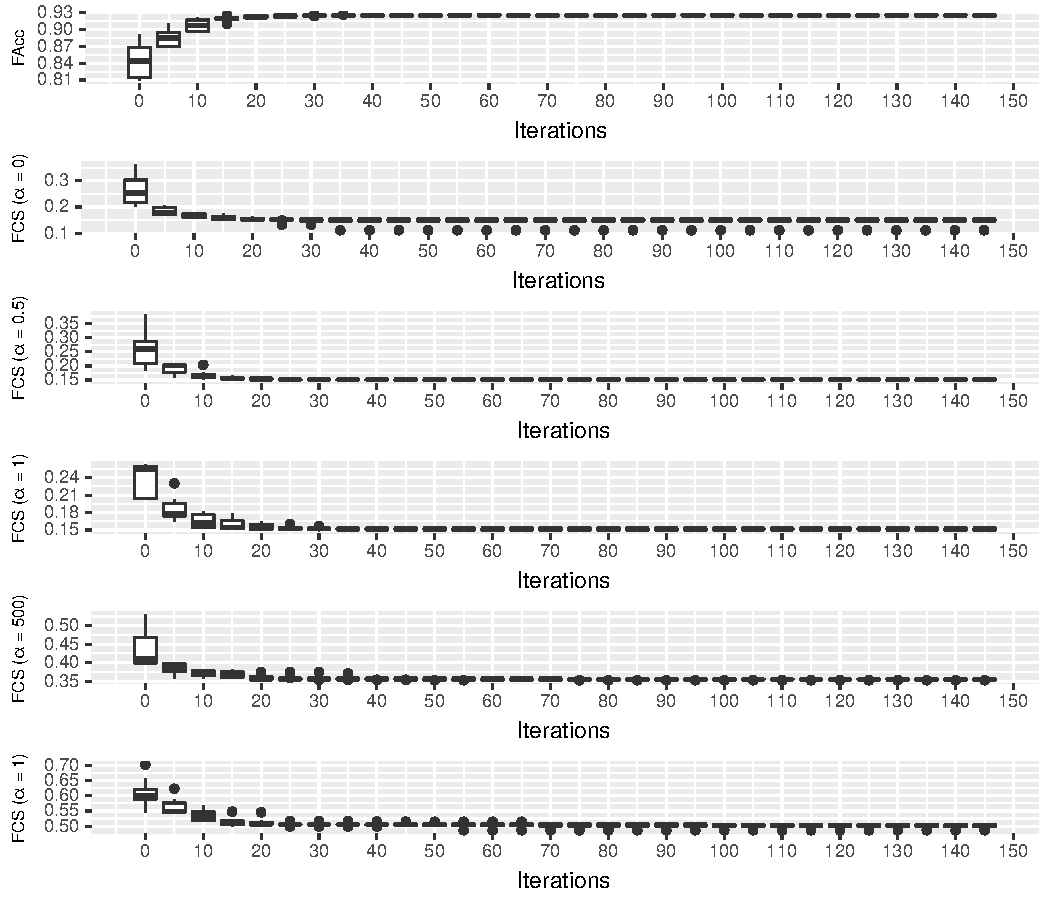
\includegraphics[width=0.8\textwidth]{img/pittsburghItvsF.pdf}
\caption{Convergence of fitness for each one of the tested fitness functions, and for Pittsburgh approach. Note that $f_{Acc}$ has to be maximised, whereas $f_{CS}$ has to be minimised.} % You know what I think about these graphs, from this one to the third. Using boxplots only makes them a bit more confusing. Boxplots should be used for comparing categories or factors. - JJ

\label{fig:pittsburghItvsF}
\end{figure*}

For the sake of clarity, $f_{CS}$ has been divided by the maximum value -- the number of instances for training -- it might take. By looking at the Pittsburgh approach values in Figure \ref{fig:pittsburghItvsF}, we see that mostly all configurations tend to converge around iteration 40, but it seems that $f_{CS}$ with $\alpha = 0.5$ is the configuration that reaches the best solution faster, around the 30th iteration.

\begin{figure*}[h!tb]
	\centering
	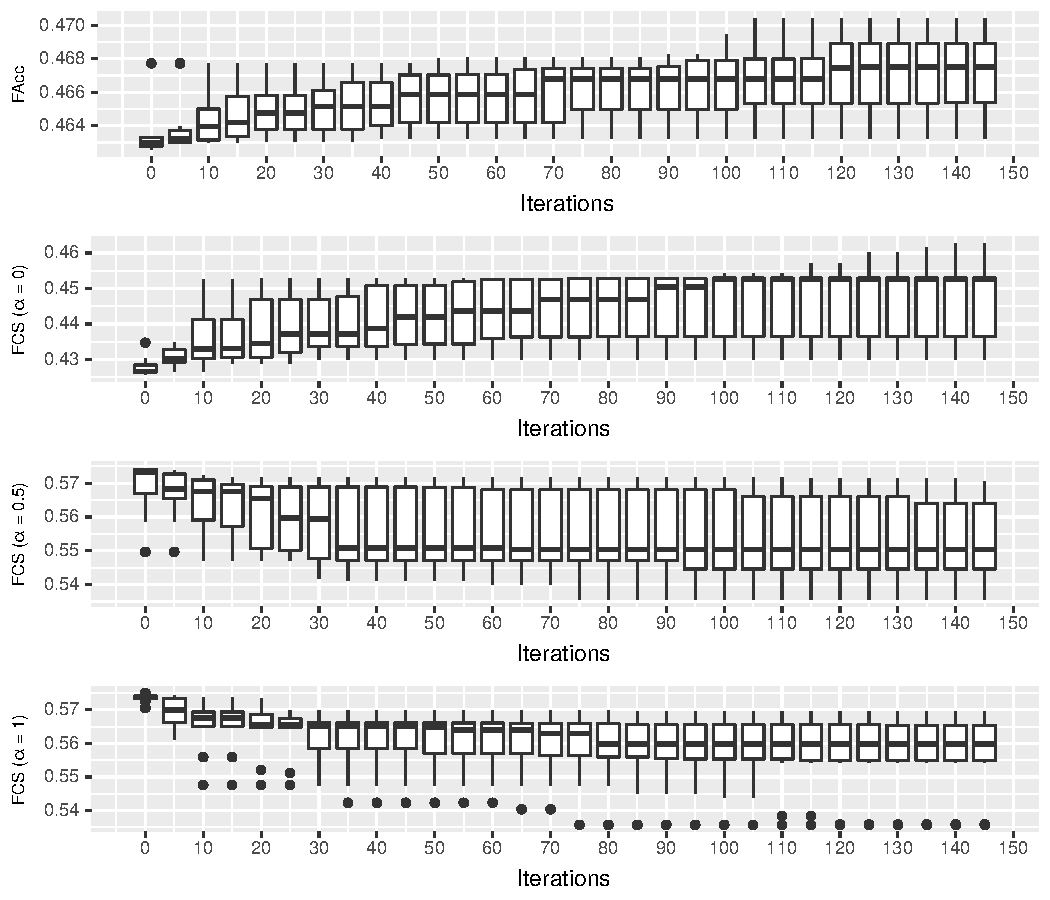
\includegraphics[width=0.8\textwidth]{img/michiganItvsF_allow.pdf}
	\caption{Convergence of fitness for each one of the tested fitness functions, and for Michigan approach being executed for the GRANTED class. Note that $f_{Acc}$ has to be maximised, whereas $f_{CS}$ has to be minimised.}
	\label{fig:michiganItvsF_allow}
\end{figure*}

With regard to the Michigan approach, a higher variability is noticeable in Figures \ref{fig:michiganItvsF_allow} and \ref{fig:michiganItvsF_deny}, but in average we see that for $f_{CS}$ with $\alpha = 0$ or 1, the fitness do not converge until generation 120. The best ones are for $f_{Acc}$ and $f_{CS}$ with $\alpha = 0.5$, being the latter the one that converges faster, around the 50th iteration.

\begin{figure*}[h!tb]
	\centering
	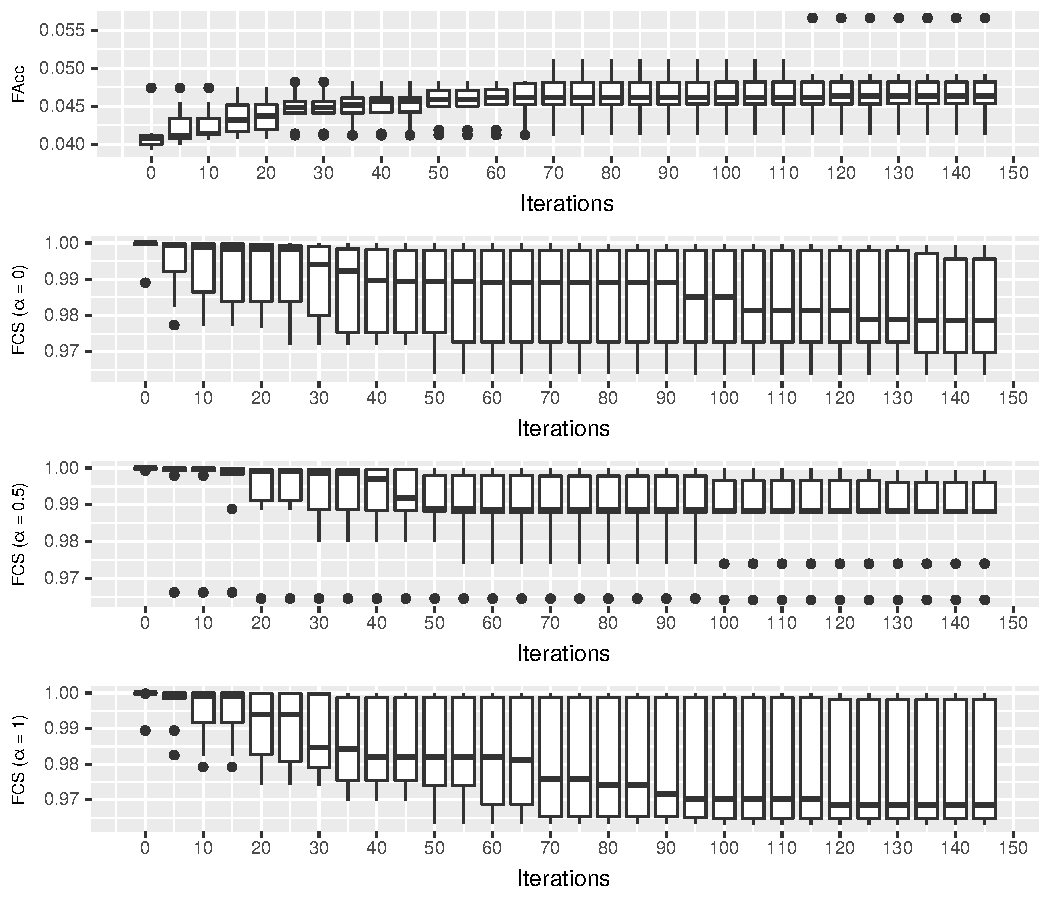
\includegraphics[width=0.8\textwidth]{img/michiganItvsF_deny.pdf}
	\caption{Convergence of fitness for each one of the tested fitness functions, and for Michigan approach being executed for the STRONGDENY class. Note that $f_{Acc}$ has to be maximised, whereas $f_{CS}$ has to be minimised.}
	\label{fig:michiganItvsF_deny}
\end{figure*}

We can advance that the best results might be obtained for $f_{CS}$ with $\alpha = 0.5$. However, as it can be seen that there is a considerable difference between the performance, in terms of best obtained fitness, of the two used approaches, we have to thoroughly compare them.

\subsection{The Pittsburgh vs. Michigan approach} % Same, not convinced, as with anything I do now.
\label{subsec:approachcomparison}

What we also have to determine is which kind of presented solution is better: showing the CSO a set of rules or a single rule for each class. As already discussed in Section \ref{sec:methodology}, each one has their advantages and disadvantages, but now we directly compare the values obtained for both implementations. Table \ref{tab:PvsMfitness} shows the results from the evaluations with $f_{Acc}$ and also $f_{CS}$.

\begin{table*}
\centering
\resizebox{16cm}{!}{
\begin{tabular}{llll|l|l|l|l|}
\cline{5-8}
                                                                          &                                                         &                                                &                & Average              & Best  & Median & Worst \\ \hline
\multicolumn{2}{|l|}{\multirow{4}{*}{Pittsburgh - individual eq. set of rules}}                                                     & \multicolumn{2}{l|}{$f_{Acc}$}                                  & 0.925 $\pm$ 0.043e-2 & 0.926 & 0.925  & 0.924 \\ \cline{3-8} 
\multicolumn{2}{|l|}{}                                                                                                              & \multicolumn{1}{l|}{\multirow{3}{*}{$f_{CS}$}} & $\alpha$ = 0   & 0.138 $\pm$ 2.153e-2 & 0.097 & 0.149  & 0.151 \\ \cline{4-8} 
\multicolumn{2}{|l|}{}                                                                                                              & \multicolumn{1}{l|}{}                          & $\alpha$ = 0.5 & 0.15 $\pm$ 0.103e-2  & 0.148 & 0.15   & 0.151 \\ \cline{4-8} 
\multicolumn{2}{|l|}{}                                                                                                              & \multicolumn{1}{l|}{}                          & $\alpha$ = 1   & 0.148 $\pm$ 0.383e-2 & 0.139 & 0.15   & 0.151 \\ \hline
\multicolumn{1}{|l|}{\multirow{8}{*}{Michigan - individual eq. one rule}} & \multicolumn{1}{l|}{\multirow{4}{*}{Class: GRANTED}}    & \multicolumn{2}{l|}{$f_{Acc}$}                                  & 0.468 $\pm$ 0.264e-2 & 0.47  & 0.468  & 0.463 \\ \cline{3-8} 
\multicolumn{1}{|l|}{}                                                    & \multicolumn{1}{l|}{}                                   & \multicolumn{1}{l|}{\multirow{3}{*}{$f_{CS}$}} & $\alpha$ = 0   & 0.555 $\pm$ 1.086e-2 & 0.543 & 0.549  & 0.572 \\ \cline{4-8} 
\multicolumn{1}{|l|}{}                                                    & \multicolumn{1}{l|}{}                                   & \multicolumn{1}{l|}{}                          & $\alpha$ = 0.5 & 0.553 $\pm$ 1.309e-2 & 0.535 & 0.55   & 0.57  \\ \cline{4-8} 
\multicolumn{1}{|l|}{}                                                    & \multicolumn{1}{l|}{}                                   & \multicolumn{1}{l|}{}                          & $\alpha$ = 1   & 0.557 $\pm$ 1.231e-2 & 0.536 & 0.56   & 0.57  \\ \cline{2-8} 
\multicolumn{1}{|l|}{}                                                    & \multicolumn{1}{l|}{\multirow{4}{*}{Class: STRONGDENY}} & \multicolumn{2}{l|}{$f_{Acc}$}                                  & 0.047 $\pm$ 0.404e-2 & 0.057 & 0.046  & 0.041 \\ \cline{3-8} 
\multicolumn{1}{|l|}{}                                                    & \multicolumn{1}{l|}{}                                   & \multicolumn{1}{l|}{\multirow{3}{*}{$f_{CS}$}} & $\alpha$ = 0   & 0.982 $\pm$ 1.41e-2  & 0.964 & 0.979  & 0.999 \\ \cline{4-8} 
\multicolumn{1}{|l|}{}                                                    & \multicolumn{1}{l|}{}                                   & \multicolumn{1}{l|}{}                          & $\alpha$ = 0.5 & 0.988 $\pm$ 1.12e-2  & 0.964 & 0.988  & 0.999 \\ \cline{4-8} 
\multicolumn{1}{|l|}{}                                                    & \multicolumn{1}{l|}{}                                   & \multicolumn{1}{l|}{}                          & $\alpha$ = 1   & 0.979 $\pm$ 1.744e-2 & 0.963 & 0.969  & 1     \\ \hline
\end{tabular}
}
\caption{Fitness comparison between Pittsburgh and Michigan
  approaches. Note that in the case of $f_{Acc}$, the best value is
  highest, whilst for $f_{CS}$, the lower is better. An $*$ indicates
  the  statistically significant best value for $\alpha$.}
% You can't compare measures that not even evaluate different things,
% but go in opposite directions (one is lower-is-better and the other
% is bigger-is-better). Classes also have different levels, so no
% comparison. Alphas have an influence in the measure, so you can't
% compare them either. Either you use a single measure to compare all
% of them, or this is simply not a comparison, by definition - JJ
\label{tab:PvsMfitness}
\end{table*}

%\subsection{Pittsburgh approach}
%
%The best obtained fitness when coding the individuals as sets of rules are detailed in Table \ref{tab:pittsburgh}. Because the algorithm has been executed 10 times, the data folded in a different way each, we obtained 10 best fitness, from which we present the worst case, the best case, and the median. It is important to point out that in the case of $F_{Acc}$ the best value is the maximum, whilst for $F_{CS}$, the best possible value is the minimum.
%
%\begin{table*}
%\begin{center}
%\begin{tabular}{cc|l|l|l|l|l|}
%\cline{3-7}
%                                                &                & Average & SD & Best       & Median & Worst \\ \hline
%\multicolumn{2}{|c|}{$F_{Acc}$}                                  & 0.925   & $<$0.001 & 0.926      & 0.925  & 0.924 \\ \hline
%\multicolumn{1}{|c|}{\multirow{3}{*}{$F_{CS}$}} & $\alpha$ = 0 *  & 7102.2  & 320.260 & 6198        & 7193   & 7253 \\ \cline{2-7} 
%\multicolumn{1}{|c|}{}                          & $\alpha$ = 0.5 & 7235.95 & 41.825 & 7149       & 7250   & 7274 \\ \cline{2-7} 
%\multicolumn{1}{|c|}{}                          & $\alpha$ = 1   & 7192.8  & 204.872 & 6620       & 7253.5 & 7298 \\ \hline
%\end{tabular}
%\caption{Best fitness obtained when the individual is coded as a set
%  of rules, following the Pittsburgh approach, and with 10-fold
%  cross-validation. Two different fitness functions have been used,
%  and for $\alpha$ values of 0, 0.5, and 1. Note that in the case of
%  $F_{Acc}$ higher is better, whilst for $F_{CS}$, the lower is
%  better. An $*$ indicates the  statistically significant best value
%  for $\alpha$.
%}
%\label{tab:pittsburgh}
%\end{center}
%\end{table*}
%% I have been looking at these tables for a while and I can't make head or tails of them. Let's see what I don't understand individually, then collectively
%% 3 and 4: I need units. Facc lists an average of 0.925 and then 7100. I have no idea if they can be compared with each other. Best and median, of what? You can use the top left corner to "title" the table. Also, you have to say in the caption what we are looking for. Are we comparing Facc with Fcs? In 4, i would expand FN and FP maybe merge columns. I can do that, no problem. But I still need the units. I am not sure we want to put that as a result. Maybe as a conclusion we could say that all errors are false positives, which, in principle, might be good: you are keeping company secrets alright.
%% Then, all together. I really don't know what you are representing here. One says "fitness" other "validation". Both say Pittsburgh. If you are comparing different representations, the tables should be merged, because you are comparing different representations. Besides, one has the FP/FN and the other does not. If you are comparing results for both representations, either you include them in both or you don't. If the results are pretty much the same, don't include them and just name them, along with saying that all data can be taken from the repo. You can publish it in FigShare too. 
%
%In the case of $F_{Acc}$ for the Pittsburgh approach, since the
%distributions do not follow the normal, a non-parametric test
%(Kruskal-Wallis) has been used to asset the statistical significance
%\cite{DerracTests11}, obtaining a p-value of 0.0001. $\alpha$ = 0 is
%significantly different with $\alpha$ = 0.5 and $\alpha$ = 1, while
%there are not differences between the two former (p-value = 0.08).
%%this is an enumeration of results. What can you say about them? Do
%%they prove your initial hypothesis? - JJ
%% Please check these questions - JJ
%
%\begin{table*}
%\begin{center}
%\begin{tabular}{cc|l|l|l|l|l|l|l|}
%\cline{3-9}
%                                                &                & Average & SD & Best       & Median & Worst & FP (avg) & FN (avg)   \\ \hline
%\multicolumn{2}{|c|}{$F_{Acc}$}                                  & 0.925 & 0.004 & 0.929      & 0.926  & 0.917 & 400.3 & 0 \\ \hline
%\multicolumn{1}{|c|}{\multirow{3}{*}{$F_{CS}$}} & $\alpha$ = 0 *  & 0.926 & 0.006 & 0.941     & 0.926   & 0.917 & 390.7 & 1.7 \\ \cline{2-9} 
%\multicolumn{1}{|c|}{}                          & $\alpha$ = 0.5 & 0.925 & 0.004 & 0.929       & 0.926   & 0.917 & 400.5 & 0 \\ \cline{2-9} 
%\multicolumn{1}{|c|}{}                          & $\alpha$ = 1   & 0.922  & 0.008 & 0.929       & 0.924 & 0.902 & 398.1 & 0 \\ \hline
%\end{tabular}
%\caption{Best validation obtained for each case, for a different fitness function or configuration has been used, and for Pittsburgh approach. They are represented by their mean and median due to the 10-fold cross-validation used. An $*$ indicates the  statistically significant best value for $\alpha$. False positives (FP) and false negatives (FN) rates are also indicated.}
%\label{tab:pittsburghVAL}
%\end{center}
%\end{table*}
%
%Taking into consideration the infrastructure available for the experiments (see Section\ref{sec:experiments}), the execution times for the Pittsburgh approach are in Table \ref{tab:pittsburghTime}, detailed by their average value and standard deviation (sd). Values are expressed in miliseconds, and it can be seen that it mostly takes the same to execute all of them, given that the stopping criterion is to finish 150 generations.
%
%\begin{table*}
%\begin{center}
%\begin{tabular}{ll|l|l|}
%\cline{3-4}
%                                                &                & Time (ms) (avg) & Time (sd)   \\ \hline
%\multicolumn{2}{|l|}{$F_{Acc}$}                                  & 18298103.6      & 6478003.741 \\ \hline
%\multicolumn{1}{|l|}{\multirow{3}{*}{$F_{CS}$}} & $\alpha$ = 0   & 18655785.8      & 5969635.164 \\ \cline{2-4} 
%\multicolumn{1}{|l|}{}                          & $\alpha$ = 0.5 & 14697743.3      & 4071043.748 \\ \cline{2-4} 
%\multicolumn{1}{|l|}{}                          & $\alpha$ = 1   & 16992321.8      & 4155989.808 \\ \hline
%\end{tabular}
%\caption{Average execution time for every kind of fitness function for the
%  Pittsburgh approach.}
%% You _really_ have to explain this a little bit more. First and
%% foremost, tables are for comparing and assessing things. You
%% probably want to compare times between the Pittsburgh and the
%% Michigan approach, so they should go together. And in general and as
%% said above, figures should be as self-contained as possible.
%% More issues
%% * I really have no idea why there are different times for GRANTED
%% and STRONGDENY. Are they different kind of fitness functions?
%% * The existence of the table itself. Are you really comparing times?
%% Is it critical in some way? If the objective is to minimize error
%% rates, as long as time is pretty much the same, it is not big deal.
%% * Avgs and std devs go together in the same column with � and using as
%% many significant digits as needed. But this point is moot, because
%% the table should leave anyway. Please remember that tables are not
%% there to add one more paragraph saying "The results are on table
%% whatever". They are to support your point or objective and to
%% compare results. 
%\label{tab:pittsburghTime}
%\end{center}
%\end{table*}
%
%\subsection{Michigan approach}
%\label{subsec:michigan}
%
%\begin{table*}
%\begin{center}
%\begin{tabular}{cc|l|l|l|l|l|l|}
%\cline{3-8}
%                                                &                                 & Class      & Average & SD & Best & Median & Worst \\ \hline
%\multicolumn{2}{|c|}{\multirow{2}{*}{$F_{Acc}$}}                                  & GRANTED    & 0.427 & 0.003 & 0.47 & 0.468 & 0.463 \\ \cline{3-8} 
%\multicolumn{2}{|c|}{}                                                            & STRONGDENY & 0.047 & 0.004 & 0.057 & 0.046 & 0.041 \\ \hline
%\multicolumn{1}{|c|}{\multirow{6}{*}{$F_{CS}$}} & \multirow{2}{*}{$\alpha$ = 0}   & GRANTED    & 21407.3 & 646.948 & 22200 & 21711 & 20630 \\ \cline{3-8} 
%\multicolumn{1}{|c|}{}                          &                                 & STRONGDENY & 47087.6 & 647.29 & 47939 & 46941 & 46220 \\ \cline{2-8} 
%\multicolumn{1}{|c|}{}                          & \multirow{2}{*}{$\alpha$ = 0.5} & GRANTED    & 26517.8 & 436.553 & 27360 & 26402.5 & 25685 \\ \cline{3-8} 
%\multicolumn{1}{|c|}{}                          &                                 & STRONGDENY & 47372.9 & 664.005 & 47932 & 47403 & 46247 \\ \cline{2-8} 
%\multicolumn{1}{|c|}{}                          & \multirow{2}{*}{$\alpha$ = 1}   & GRANTED    & 26724 & 502.579 & 27317 & 26853 & 25696 \\ \cline{3-8} 
%\multicolumn{1}{|c|}{}                          &                                 & STRONGDENY & 46949.3 & 588.485 & 47967 & 46455 & 46189 \\ \hline
%\end{tabular}
%\caption{Best fitness obtained when the individual is coded as a
%  single rule, following the Michigan approach, and represented by
%  class. Data was divided in 10-folds to perform cross-validation. Two
%  different fitness have been used, and for $\alpha$ values of 0, 0.5,
%  and 1. Note that in the case of $F_{Acc}$ higher is better, whilst
%  for $F_{CS}$, lower is better.}
%\label{tab:michigan}
%\end{center}
%\end{table*}
%
%%We wanted to test different values of alpha because... (hypotesis you
%%want to prove). However... 
%No significant differences have been found between the results of
%applying the % Please revise grammar thoroughly - JJ
%three values of $\alpha$, for GRANTED and STRONGDENY. % which means,
%                                % in the context of this problem,
%                                % that... 
%In the case of comparing the three distributions % Distributions or
%                                % results for different values of
%                                % alpha? 
%for STRONGDENY, an ANOVA test has been applied instead Kruskal-Wallis,
%as these distributions follow a normal curve. % and results obtained
%                                % show that.... which means... 
%                                
%\begin{table*}
%\begin{center}
%\begin{tabular}{cc|l|l|l|l|l|l|l|l|}
%\cline{3-10}
%                                                &                                 & Class      & Average & SD & Best & Median & Worst & FP (avg) & FN (avg) \\ \hline
%\multicolumn{2}{|c|}{\multirow{2}{*}{$F_{Acc}$}}                                  & GRANTED    & 0.467 & 0.004 & 0.472 & 0.468 & 0.459 & 112.3  & 0 \\ \cline{3-10} 
%\multicolumn{2}{|c|}{}                                                            & STRONGDENY & 0.046 & 0.007 & 0.065 & 0.045 & 0.037 & 0 & 25.5 \\ \hline
%\multicolumn{1}{|c|}{\multirow{6}{*}{$F_{CS}$}} & \multirow{2}{*}{$\alpha$ = 0}   & GRANTED    & 0.466 & 0.004 & 0.472 & 0.467 & 0.459 & 110.6 & 0 \\ \cline{3-10} 
%\multicolumn{1}{|c|}{}                          &                                 & STRONGDENY & 0.024 & 0.015 & 0.045 & 0.023 & 0.003 & 0 & 473.8 \\ \cline{2-10} 
%\multicolumn{1}{|c|}{}                          & \multirow{2}{*}{$\alpha$ = 0.5} & GRANTED    & 0.467 & 0.003 & 0.472 & 0.467 & 0.462 & 116.9 & 0 \\ \cline{3-10} 
%\multicolumn{1}{|c|}{}                          &                                 & STRONGDENY & 0.02 & 0.016 & 0.061 & 0.015 & 0.002 & 0 & 188.8 \\ \cline{2-10} 
%\multicolumn{1}{|c|}{}                          & \multirow{2}{*}{$\alpha$ = 1}   & GRANTED    & 0.465 & 0.004 & 0.472 & 0.466 & 0.458 & 161.2 & 0 \\ \cline{3-10} 
%\multicolumn{1}{|c|}{}                          &                                 & STRONGDENY & 0.025 & 0.019 & 0.047 & 0.036 & 0 & 0 & 1274.5 \\ \hline
%\end{tabular}
%\caption{Best validation obtained for each case, for a different fitness function or configuration has been used, and for Michigan approach. They are represented by their mean and median due to the 10-fold cross-validation used. An $*$ indicates the  statistically significant best value for $\alpha$. False positives (FP) and false negatives (FN) rates are also indicated.}
%\label{tab:michiganVAL}
%\end{center}
%\end{table*}
%% Tables are for presenting information and to make the reader assess
%% your method. In that sense, the Pittsburgh approach uses a single
%% run to obtain a set of rules. The Michigan approach uses two
%% runs. The reader does not care how those rules are obtained, even
%% more so if you are not comparing how fast you find the STRONGDENY
%% rule. First, you should report the results TOGETHER. Second,
%% averages shold be for the running time of the run for STRONGDENY and
%% the run for GRANT _together_, not each one separately.
%
%Furthermore, Tables \ref{tab:michigan} and \ref{tab:michiganVAL} show worse results for the class STRONGDENY than for the class GRANTED. If we analyse the ratio of instances in each class, we obtain that the majority class is indeed GRANTED, and it surpasses the STRONGDENY class in 13:1.
%
%Execution times (in average) can be consulted in Table \ref{tab:michiganTime}. It is important to understand, before making a comparison with results in Table \ref{tab:pittsburghTime} from the Pittsburgh approach, that for each different fitness or configuration of the fitness (different $\alpha$), in the Michigan approach the algorithm has to be executed twice, given that we obtain a single rule as a solution at the time we have two classes. This means that even though we can see the times described in Table \ref{tab:michiganTime} are around half the ones in Table \ref{tab:pittsburghTime}, the times for both classes should be added up together.
%
%\begin{table*}
%\begin{center}
%\begin{tabular}{lll|l|l|}
%\cline{4-5}
%                                                &                                                      &            & Time (ms) (avg) & Time (sd)   \\ \hline
%\multicolumn{2}{|l|}{\multirow{2}{*}{$F_{Acc}$}}                                                       & GRANTED    & 8425228         & 1300396.316 \\ \cline{3-5} 
%\multicolumn{2}{|l|}{}                                                                                 & STRONGDENY & 8066737.1       & 554270.509  \\ \hline
%\multicolumn{1}{|l|}{\multirow{6}{*}{$F_{CS}$}} & \multicolumn{1}{l|}{\multirow{2}{*}{$\alpha$ = 0}}   & GRANTED    & 8477672.1       & 968703.507  \\ \cline{3-5} 
%\multicolumn{1}{|l|}{}                          & \multicolumn{1}{l|}{}                                & STRONGDENY & 9186603         & 434653.670  \\ \cline{2-5} 
%\multicolumn{1}{|l|}{}                          & \multicolumn{1}{l|}{\multirow{2}{*}{$\alpha$ = 0.5}} & GRANTED    & 8190161.6       & 781166.295  \\ \cline{3-5} 
%\multicolumn{1}{|l|}{}                          & \multicolumn{1}{l|}{}                                & STRONGDENY & 8417774.8       & 671246.764  \\ \cline{2-5} 
%\multicolumn{1}{|l|}{}                          & \multicolumn{1}{l|}{\multirow{2}{*}{$\alpha$ = 1}}   & GRANTED    & 9274908.1       & 1309297.086 \\ \cline{3-5} 
%\multicolumn{1}{|l|}{}                          & \multicolumn{1}{l|}{}                                & STRONGDENY & 8955486.7       & 835676.926  \\ \hline
%\end{tabular}
%\caption{Average execution time for each used fitness for the
%  Pittsburgh approach.}
%% Besides all I've said above, "sd" can't be labelled "time". You
%% should really put them in the same column. 
%\label{tab:michiganTime}
%\end{center}
%\end{table*}

\subsection{Examples of the best obtained individuals}
\label{subsec:examples}

Once the results have been analysed, here we present some examples of the individuals that have been obtained in the simulations, proving their readability and usefulness for the CSOs. In addition, we present the relation between the obtained solutions and the original rules that allowed to classify the dataset we have been working with.

% You can't introduce in the results section something completely
% unrelated to the stated objective of the paper. Nowhere you have
% said you were going to compare different types of fitness, or
% different "alphas" - JJ

\section{Conclusions and Future Work}
\label{sec:future}

% (Paloma) From now on, please take into consideration that finished sections will be sent for review. If they are not under review it's because they are not finished.
% General layout of conclusions
% We wanted to do this with this motivation.
% We have done this and that in this paper and met objective 1 and 2 or answered research question 1 and 2; however, we think that question 3 has not been answered properly
% We think we could answer question 3 properly if we did this and that. Which is left as future work.

% You can't refer to other sections in conclusions. Conclusions exist just because reviewers are lazy and just look at the abstract, the pretty pictures and conclusions. If you make them go elsewhere and they are not self-contained, reviewer #3 is going to make you pay dearly.
As it has been seen in Sections \ref{subsec:michigan} and \ref{subsec:examples}, the highly imbalanced data set that we are
% This is also the first time you talk about imbalance. It is is simply not in the title, abstract, introduction or conclusion and thus it is simply not part of the paper. You can say you didn't meet your objectives in something that is _not_ an objective, but if that's the case, it opens an attack angle for reviewer #3, who will say "Why don't you address the imbalanced data set?" carrying us along to a second round of experiments, major rewriting, and so on. Conclusions must constrain themselves to the stated objectives of the paper. Have you created a decision-aid system that simplifies CSO rules? Check. That's it. You have tried several things, which one do you think would be the best? Can you generalize this to non-byod non-security environments? In which case? Those are the ocnclusions. 
using clearly biases the results towards the majority class 
\cite{japkowicz2002class}, in this case, GRANTED. In this sense,
solutions can be found in literature in order to reduce the bias while
performing classification tasks, such as in \cite{chawla2005data} and
\cite{sun2009classification}. Also, in \cite{bhowan2012developing},
the authors present a comparison between many different types of
fitness functions, testing on various unbalanced datasets, with
different minority-class/majority-class ratios. For our future work we
will implement these solutions to continue improving our system. 
%Conclusions don't usually include references, either. They can, if you say something like "well, we could do things along this path in the future". But the way it is written now, it sounds like something you _should_ have done in this paper but had not actually done. You will probably add more stuff in the future, but right now the only thing you  have is a negative conclusion, which is not nearly enough.

\section*{Acknowledgments.}

This work has been supported in part by TIN2014-56494-C4-3-P (Spanish
Ministry of Economy and Competitivity), PROY-PP2015-06 (Plan Propio
2015 UGR). %Is this one still working? - JJ

\bibliographystyle{elsarticle-num}
\bibliography{GPrules,geneura}

\end{document}
